\documentclass{article}

\usepackage{tikz}

\begin{document}

\begin{figure}
  \centering
  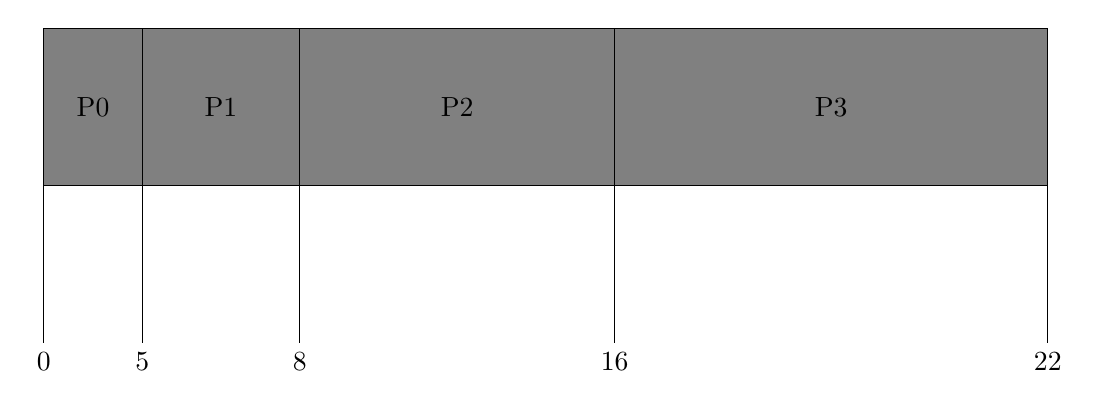
\begin{tikzpicture}[xscale=0.25]
    % 5
    \draw [fill=gray] (0,0) rectangle (5,2);
    \node at (2.5,1) {P0};
    \draw [-] (0,0) -- (0,-2);
    \node [below] at (0,-2) {0};
    % 8
    \draw [fill=gray] (5,0) rectangle (13,2);
    \node at (9,1) {P1};
    \draw [-] (5,0) -- (5,-2);
    \node [below] at (5,-2) {5};
    % 16
    \draw [fill=gray] (13,0) rectangle (29,2);
    \node at (21,1) {P2};
    \draw [-] (13,0) -- (13,-2);
    \node [below] at (13,-2) {8};
    % 22
    \draw [fill=gray] (29,0) rectangle (51,2);
    \node at (40,1) {P3};
    \draw [-] (29,0) -- (29,-2);
    \node [below] at (29,-2) {16};
    % end
    \draw [-] (51,0) -- (51,-2);
    \node [below] at (51,-2) {22};
  \end{tikzpicture}
\end{figure}

\end{document}
